\section{Moment-cumulant relations in noncommutative probability}\label{sec:momentcumulantrel}

\subsection{Noncrossing partitions}

Partitions and noncrossing partitions are fundamental objects in the combinatorial study of noncommutative probability theory.
\begin{Definition}\quad
\begin{enumerate}\itemsep=0pt
\item Recall that a \textit{noncrossing partition} of $[n] = \{1,\dots,n\}$ is a set partition $\pi = \{V_1,\dots,V_k\}$ of $[n]$ such that there are no elements $a<b<c<d$ in $[n]$ such that $a,c \in V_i$ and $b,d \in V_j$, and $i\neq j$. The elements of $\pi$ are called the \textit{blocks of $\pi$}. We denote by $\NC(n)$ to the set of noncrossing partitions of $[n]$.
\item We say that $\pi \in \NC(n)$ is \textit{irreducible} if both $1$ and $n$ belong to the same block in $\pi$. We will write $\NC_{\mathrm{irr}}(n)$ to denote the set of irreducible noncrossing partitions on~$[n]$.
\item An \textit{interval partition} is a noncrossing partition $\pi\in\NC(n)$ such that all its blocks are of the form $\{k,k+1,\dots,k+l\}$ for some $1\leq k\leq n$ and $0\leq l\leq n-k$. The set of interval partitions of $[n]$ is denoted $\Int(n)$.
\end{enumerate}
\end{Definition}

\begin{figure}[t]
$$
\begin{array}{c c c}
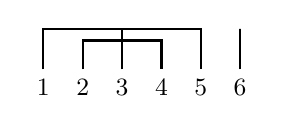
\begin{tikzpicture}[thick,font=\small]
 \path 	(0,0) 		node (a) {1}
 	(0.5,0) 	node (b) {2}
 	(1,0) 		node (c) {3}
 	(1.5,0) 	node (d) {4}
 	(2,0) 		node (e) {5}
	(2.5,0) 		node (f) {6};
 \draw (a) -- +(0,0.75) -| (e);
 \draw (b) -- +(0,0.60) -| (d);
 \draw (c) -- +(0,0.75) -| (c);
 \draw (f) -- +(0,0.75) -| (f);
 \end{tikzpicture}
 & \quad &
 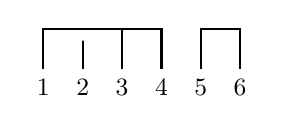
\begin{tikzpicture}[thick,font=\small]
 \path 	(0,0) 		node (a) {1}
 	(0.5,0) 	node (b) {2}
 	(1,0) 		node (c) {3}
 	(1.5,0) 	node (d) {4}
 	(2,0) 		node (e) {5}
 	(2.5,0) 	node (f) {6};
 \draw (a) -- +(0,0.75) -| (d);
 \draw (c) -- +(0,0.75) -| (c);
 \draw (b) -- +(0,0.60) -| (b);
 \draw (e) -- +(0,0.75) -| (f);
 \end{tikzpicture}\\
 \mbox{a) Crossing partition}& \quad & \mbox{b) Noncrossing partition}\\[0.2cm]
 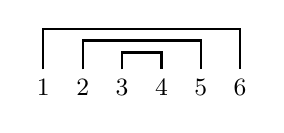
\begin{tikzpicture}[thick,font=\small]
 \path 	(0,0) 		node (a) {1}
 	(0.5,0) 	node (b) {2}
 	(1,0) 		node (c) {3}
 	(1.5,0) 	node (d) {4}
 	(2,0) 		node (e) {5}
 	(2.5,0) 	node (f) {6};
 \draw (a) -- +(0,0.75) -| (f);
 \draw (b) -- +(0,0.60) -| (e);
 \draw (c) -- +(0,0.45) -| (d);
 \end{tikzpicture}
 & \quad &
 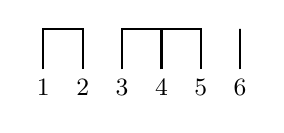
\begin{tikzpicture}[thick,font=\small]
 \path 	(0,0) 		node (a) {1}
 	(0.5,0) 	node (b) {2}
 	(1,0) 		node (c) {3}
 	(1.5,0) 	node (d) {4}
 	(2,0) 		node (e) {5}
 	(2.5,0) 	node (f) {6};
 \draw (a) -- +(0,0.75) -| (b);
 \draw (c) -- +(0,0.75) -| (e);
 \draw (d) -- +(0,0.75) -| (d);
 \draw (f) -- +(0,0.75) -| (f);
 \end{tikzpicture}
 \\ \mbox{c) Irreducible partition} &\quad &\mbox{d) Interval partition}
\end{array}
$$
\caption{Different types of set partitions of the set $[6]=\{1,\dots,6\}$.}
\end{figure}

The set $\NC(n)$ is endowed with a poset structure as follows: for two partitions $\pi,\sigma \in \NC(n)$, we say that $\pi \leq \sigma$ if and only if every block in $\pi$ is contained in a block of $\sigma$. This order is called the \textit{reverse refinement order} on $\NC(n)$. It provides a lattice structure on $\NC(n)$, with maximal element being the partition into a single block, $1_n = \{\{1,\dots,n\}\}$, and the minimal element consisting of $n$ blocks, $0_n = \{ \{1\},\dots, \{n\}\}$.

For every noncrossing partition $\pi = \{V_1,\dots,V_k\}\in \NC(n)$, we can define an order on the blocks by stating that for $V_{i_s},V_{i_t} \in \pi$, $V_{i_s}\leq V_{i_t}$ if only if $V_{i_t}$ is nested in $V_{i_s}$, i.e., $a \in [\min{V_{i_s}},\max{V_{i_s}}]$ for any $a \in V_{i_t}$. It is clear that the maximal elements in~$\pi$ are the interval blocks.
Given a minimal block $V\in \pi\in \NC(n)$, we say that $\pi':=\{ W\in \pi\colon W\leq V\}$ is an \textit{irreducible component of~$\pi$}. In other words, $\pi'$ is a noncrossing partition obtained by restricting~$\pi$ to the interval $[\min(V),\max(V)]$. It is clear then that $\pi$ has a unique irreducible component if and only if $\pi$ is an irreducible noncrossing partition.

Associated to an irreducible noncrossing partition $\pi\in \NC_{\mathrm{irr}}(n)$, we can construct a rooted tree $t(\pi)$ with $|\pi| = k$ vertices. The vertices of $t(\pi)$ are decorated by the blocks of $\pi$, and there is a directed edge from a vertex $v$ to a vertex $w$ if and only if the corresponding block $V$ associated to $v$ \textit{covers} the block $W$ associated to $w$, i.e.~$V<W$ and there is no other block $U\in \pi$ such that $V<U<W$. The tree $t(\pi)$ is called the \textit{tree of nestings} of~$\pi$. For the general case of $\pi \in \NC(n)$, we define the \textit{forest of nestings of~$\pi$}, also denoted by~$t(\pi)$. It consists of the ordered forest of rooted trees of nestings of the irreducible components of~$\pi$, where the order of the irreducible components is given by the total order determined by the minimum element of each component.

The \emph{tree factorial} is recursively defined for any rooted tree $t$ by $t! = 1$ if $t$ is the rooted tree consisting of a single vertex. Otherwise, if $t$ is a rooted tree that can be obtained by grafting the subtrees $s_1,\dots,s_m$ to the root vertex, i.e., $t=[s_1,\dots,s_m]$, then
$t! = |s| s_1!\cdots s_m!$.
Here, the degree $|t|=1+|s_1| + \cdots + |s_m|$ of $t$ is its number of vertices. Finally, if $f$ is a forest formed by rooted trees $t_1,\dots,t_m$, we define $f! := t_1!\cdots t_m!$.

\begin{figure}[h]
$$
\begin{array}{c@{\,}c@{\,} c c @{\,}c@{\,} c}
\pi &=& 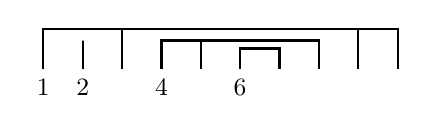
\begin{tikzpicture}[baseline={([yshift=0.3ex]current bounding box.center)},thick,font=\small]
 \path 	(0,0) 		node (a) {1}
 	(0.5,0) 	node (b) {2}
 	(1,0) 		node (c) {\phantom{1}}
 	(1.5,0) 	node (d) {4}
 	(2,0) 		node (e) {\phantom{1}}
 	(2.5,0) 	node (f) {6}
 	(3,0) 		node (g) {\phantom{1}}
 	(3.5,0) 	node (h) {\phantom{1}}
		(4,0) 		node (i) {\phantom{1}}
		(4.5,0) 	node (j) {\phantom{1}};
 \draw (a) -- +(0,0.75) -| (j);
 \draw (b) -- +(0,0.60) -| (b);
 \draw (c) -- +(0,0.75) -| (c);
 \draw (d) -- +(0,0.60) -| (e);
 \draw (e) -- +(0,0.60) -| (h);
 \draw (f) -- +(0,0.50) -| (g);
 \draw (i) -- +(0,0.75) -| (j);
 \end{tikzpicture}, 	& \quad t(\pi) &=&
				 \begin{tikzpicture}[baseline={([yshift=-1ex]current bounding box.center)},scale=0.6,
level 1/.style={level distance=7mm,sibling distance=7mm}]
\node(0)[solid node,label=right:{\tiny 1}]{}
child{node(1)[solid node,label=left:{\tiny 2}]{}
}
child{node(2)[solid node,label=right:{\tiny 4}]{}
	child{[black] node(11)[solid node,label=right:{\tiny 6}]{}}
};
\end{tikzpicture}
\\[5mm]
\sigma &= & 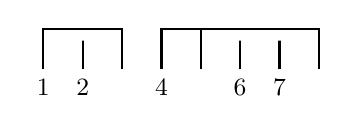
\begin{tikzpicture}[baseline={([yshift=0.3ex]current bounding box.center)},thick,font=\small]
 \path 	(0,0) 		node (a) {1}
 	(0.5,0) 	node (b) {2}
 	(1,0) 		node (c) {\phantom{1}}
 	(1.5,0) 	node (d) {4}
 	(2,0) 		node (e) {\phantom{1}}
 	(2.5,0) 	node (f) {6}
 	(3,0) 		node (g) {7}
 	(3.5,0) 	node (h) {\phantom{1}};
 \draw (a) -- +(0,0.75) -| (c);
 \draw (b) -- +(0,0.60) -| (b);
 \draw (c) -- +(0,0.75) -| (c);
 \draw (d) -- +(0,0.75) -| (e);
 \draw (e) -- +(0,0.75) -| (h);
 \draw (f) -- +(0,0.60) -|(f);
 \draw (g) -- +(0,0.60)-|(g);
 \end{tikzpicture}, 	& \quad t(\sigma) &=&\;\;\begin{tikzpicture}[baseline={([yshift=-1ex]current bounding box.center)},scale=0.6,
level 1/.style={level distance=7mm,sibling distance=7mm}]
\node(0)[solid node,label=right:{\tiny 1}]{}
child{node(1)[solid node,label=right:{\tiny 2}]{}
};
\end{tikzpicture}
\;\; \begin{tikzpicture}[baseline={([yshift=-1ex]current bounding box.center)},scale=0.6,
level 1/.style={level distance=7mm,sibling distance=7mm}]
\node(0)[solid node,label=right:{\tiny 4}]{}
child{node(1)[solid node,label=left:{\tiny 6}]{}
}
child{node(2)[solid node,label=right:{\tiny 7}]{}
};
\end{tikzpicture}
\end{array}
$$
\caption{Noncrossing partitions $\pi$ and $\sigma$ together with their respective forest of nesting $t(\pi)$ and $t(\sigma)$. Each vertex of the forest is decorated with the minimal element of their associated block in the partition.}
\end{figure}

\subsection{Cumulants in noncommutative probability}\label{sec:cumulants}

As stated in the introduction, cumulants are an important tool for dealing with noncommutative notions of independence. Before recalling the definition of cumulants, we fix some notation.
\begin{Definition}
 Let $\A$ be a vector space and let $\{f_n\colon \A^n \to \mathbb{C}\}_{n\geq1}$ be a family of multilinear functionals. For each $\pi \in \NC(n)$ and elements $a_1,\dots,a_n \in \A$, we denote{\samepage
\[
	f_{\pi}(a_1,\dots,a_n) := \prod_{V \in \pi} f_{|V|}(a_1,\dots,a_n | V),
\]
where for $V = \{i_1 < \cdots < i_s\}$, $f_{|V|}(a_1,\dots,a_n|V) := f_s(a_{i_1},\dots,a_{i_s})$.}
\end{Definition}
A \textit{noncommutative probability space} is a pair $(\A,\varphi)$ where $\A$ is a unital algebra over $\mathbb{C}$ and $\varphi\colon \A\to \mathbb{C}$ is a unital linear functional such that $\varphi(1_\A)=1$, where $1_\A$ is the unit of $\A$. In this note, we are not assuming that $\A$ or $\varphi$ have any additional structure, for instance, the existence of an involution on $\A$ or positivity of $\varphi$.
Let $(\A,\varphi)$ be a noncommutative probability space. Associated to it, we can construct a family of multilinear functionals $\{\varphi_n\colon \A^n\to\mathbb{C}\}_{n\geq 1}$ by the defining $\varphi_n(a_1,\dots,a_n) := \varphi(a_1\cdots a_n)$, for any $n\geq1$ and $a_1,\dots,a_n\in \A$. Note that $a_1\cdots a_n$ is a product in $\A$. The definition of cumulants can be stated as follows.

\begin{Definition}
Let $(\A,\varphi)$ be a noncommutative probability space.
\begin{itemize}\itemsep=0pt
\item \textit{Free cumulants} are the family of multilinear functionals $\{r_n\colon \A^n\to\mathbb{C}\}_{n\geq1}$ recursively defined by~\cite{Spe94}
\begin{equation}\label{eq:freeMC}
\varphi_n(a_1,\dots,a_n) = \sum_{\pi\in \NC(n)} r_\pi(a_1,\dots,a_n).
\end{equation}
\item \textit{Boolean cumulants} are the family of multilinear functionals $\{b_n\colon \A^n\to\mathbb{C}\}_{n\geq1}$ recursively defined by~\cite{SW97}
\begin{equation}\label{eq:BoolMC}
\varphi_n(a_1,\dots,a_n) = \sum_{\pi\in \Int(n)} b_\pi(a_1,\dots,a_n).
\end{equation}
\item \textit{Monotone cumulants} are the family of multilinear functionals $\{h_n\colon \A^n\to\mathbb{C}\}_{n\geq1}$ recursively defined by~\cite{HS11b}
\begin{equation}\label{eq:monMC}
\varphi_n(a_1,\dots,a_n) = \sum_{\pi\in \NC(n)} \frac{1}{t(\pi)!} h_\pi(a_1,\dots,a_n).
\end{equation}
\end{itemize}

\end{Definition}
Formulas \eqref{eq:freeMC}, \eqref{eq:BoolMC} and \eqref{eq:monMC} are called the \textit{free, Boolean and monotone moment-cumulant relations}, respectively.

\if

\else

Recall that for each $n\geq1$, $\NC(n)$ is a poset with respect to the reverse refinement order. Also, the restriction of this order to interval partitions gives us a poset structure on $\Int(n)$. Hence, it is possible to invert equations \eqref{eq:freeMC} and \eqref{eq:BoolMC} via M\"obius inversion in order to write the free and Boolean cumulants in terms of moments
\begin{eqnarray}
	\label{eq:freeCM}
	r_n(a_1,\dots,a_n)
	&=& \sum_{\sigma \in \NC(n)} \operatorname{M\ddot{o}b}(\sigma,1_n)\varphi_\sigma(a_1,\dots,a_n),
	\\ \label{eq:BoolCM}
	b_n(a_1,\dots,a_n)
	&=& \sum_{\sigma \in \Int(n)}(-1)^{|\sigma|-1}\varphi_\sigma(a_1,\dots,a_n),
\end{eqnarray}
where $\mathrm{M\ddot{o}b}$ stands for the M\"obius function on the incidence algebra of noncrossing partitions.
On the other hand, by using \eqref{eq:labeling} it is readily shown that the monotone moment-cumulant formula can be written as
\begin{equation}
\label{eq:monMC2}
	\varphi_n(a_1,\dots,a_n) = \sum_{\pi\in \NC(n)} \frac{1}{t(\pi)!} h_\pi(a_1,\dots,a_n),
\end{equation}
for any $a_1,\dots,a_n\in \A$. Unlike the free and Boolean cases, the coefficients $\frac{1}{t(\pi)!}$ are not multiplicative, so we cannot apply M\"obius inversion in order to express the monotone cumulants in terms of moments. The two subsequent sections of this note are devoted to describing the combinatorial tools used with the purpose of obtaining a formula analogous to \eqref{eq:freeCM} and \eqref{eq:BoolCM} for the monotone case.

\fi

\section{Shuffle approach for noncommutative probability}
\label{sec:shuffle}

In this section, we briefly describe the Hopf-algebraic framework of Ebrahimi-Fard and Patras developed in a series of recent articles \cite{EFP1, EFP2, EFP3, EFP4, EFP5}. The key ingredient in the group-theoretical framework of Ebrahimi-Fard and Patras is an unshuffle (or codendriform) structure on the double tensor algebra defined over $\A$. More precisely, given a noncommutative probability space~$(\A,\varphi)$, we consider the double tensor algebra
\[
	T(T_+(\A)) = \bigoplus_{n\geq0} T_+(\A)^{\otimes n},
	\qquad\text{where}\quad
	T_+(\A) = \bigoplus_{n\geq1} \A^{\otimes n}.
\]
In the following, we will omit the tensor symbol when denoting elements of $T_+(\A)$, that is, we consider them as words $w = a_1\cdots a_n \in \A^{\otimes n}$, where $a_1,\dots,a_n\in \A$. On the other hand, the product of words in $T(T_+(\A))$ is denoted by the bar notation, $w_1|\cdots |w_m$, where $w_1,\dots,w_m \allowbreak\in T_+(\A)$. Observe that the empty word, denoted by~$\uno$, works as the unit for the bar product. Moreover, $T(T_+(\A))$ has a multigrading and grading given by
\[
	T(T_+(\A))_{n_1,\dots,n_k}
	:= T_+(\A)^{\otimes n_1} \otimes \cdots \otimes T_+(\A)^{\otimes n_k},
\]
respectively,
\[
	T(T_+(\A))_n :=
	\bigoplus_{n_1+\cdots + n_k = n} T(T_+(\A))_{n_1,\dots,n_k},
\]
for any $n,n_1,\dots,n_k\geq1$. Additionally, we consider the algebra morphism $\epsilon\colon T(T_+(\A))\to\mathbb{C}$ defined to be zero on the augmentation ideal $T_+(T_+(\A)) = \bigoplus_{n\geq 1} T_+(\A)^{\otimes n}$ and $\epsilon(\uno) = 1$.

In order to describe the desired Hopf algebra structure on $T(T_+(\A))$, we have to present the coproduct. To this end,
 we describe the following notation. Given a subset $S\subseteq [n] :=\{1,\dots, n\}$, we define the connected components of $[n]\backslash S$ as the set of maximal intervals contained in $[n]\backslash S$. Now, given a word $w= a_1\cdots a_n$ and a subset $S = \{s_1 <\cdots < s_r\} \subseteq [n]$, we define
\[
	a_S = a_{s_1}\cdots a_{s_r},
\]
with the convention that $a_\emptyset = \uno$ (the unit of $T(T_+(\A))$). Also, if $J_1,\dots,J_r$ be the connected components of $[n] \backslash S$ ordered according to their minimum element, we denote
\[
	a_{J_{[n]}^S} = a_{J_1} | \cdots | a_{J_r}.
\]
With the above notations, we can state the desired coproduct: let $\Delta\colon T(T_+(\A))\to T(T_+(\A))\otimes T(T_+(\A))$ the algebra morphism defined by $\Delta(\uno) = \uno\otimes \uno$ and
\begin{equation}
\label{eq:copEFP}
	\Delta(a_1\cdots a_n)= \sum_{S\subseteq [n]} a_S \otimes a_{J_{[n]}^S}.
\end{equation}

\begin{Example}
For $n=4$, we have
\begin{align*}
	\Delta(a_1a_2a_3a_4)
={} & a_1a_2a_3a_4\otimes \uno + a_1 \otimes a_2a_3a_4 + a_2\otimes a_1| a_3a_4 + a_3 \otimes a_1a_2| a_4 + a_4\otimes a_1a_2a_3
	\\&\!{} + a_1a_2\otimes a_3a_4 + a_1a_3\otimes a_2|a_4 + a_1a_4\otimes a_2a_3 + a_2a_3\otimes a_1|a_4 + a_2a_4\otimes a_1|a_3
	\\&\!{} + a_3a_4\otimes a_1a_2 + a_1a_2a_3\otimes a_4 + a_1a_2a_4\otimes a_3 + a_1a_3a_4\otimes a_2 + a_2a_3a_4\otimes a_1
	\\&\!{} + \uno \otimes a_1a_2a_3a_4.
\end{align*}
\end{Example}
With the above definitions, we have the following result.

\begin{Theorem}[\cite{EFP1}]\label{thm:HopfAlg}
$(T(T_+(\A)),\Delta,\epsilon))$ is a connected graded noncommutative and noncocommutative Hopf algebra.
\end{Theorem}

The fundamental observation of the authors of \cite{EFP1} is that the coproduct defined in \eqref{eq:copEFP} can be split into two parts of the form
\[
	\Delta = \Delta_\prec + \Delta_\succ,
\]
where
\begin{gather*}
	\Delta_\prec (a_1\cdots a_n)
	= \sum_{1\in S\subseteq [n]} a_S \otimes a_{J_{[n]}^S},\qquad
 	\Delta_\succ (a_1\cdots a_n)
	= \sum_{1\not\in S\subseteq [n]} a_S \otimes a_{J_{[n]}^S}
\end{gather*}
for any word $a_1\cdots a_n\in \A^{\otimes n}$, $n\geq 1$. Both maps can be extended to $T(T_+(\A))$ by stating that
\begin{align*}
	\Delta_\prec(w_1|w_2|\cdots |w_n)
	&= \Delta_\prec(w_1)|\Delta(w_2|\cdots|w_n),\\
	\Delta_\succ(w_1|w_2|\cdots |w_n)
	&= \Delta_\succ(w_1)|\Delta(w_2|\cdots|w_n),
\end{align*}
for any words $w_1,\dots,w_n\in T_+(\A)$.

\begin{Theorem}[\cite{EFP1}]
\label{thm:unshuffle}
$(T(T_+(\A)),\Delta_\prec,\Delta_\succ)$ is a unital unshuffle bialgebra.
\end{Theorem}

Unshuffle bialgebras are also called \textit{codendriform bialgebras} \cite{Foissy}. For details, including definitions and a proof of the above theorem, we refer the reader to \cite[Theorem~5]{EFP1}.

Theorem \ref{thm:unshuffle} permits to show that the algebraic dual of $(T(T_+(\A)),\Delta,\epsilon))$ is a unital shuffle algebra. More precisely, for $f,g\in \operatorname{Lin}(T(T_+(\A)),\mathbb{C})$, we can define the associative convolution product dual to~\eqref{eq:copEFP} by
\begin{equation}\label{eq:convol}
	f*g = m_{\mathbb{C}}\circ (f\otimes g)\circ \Delta,
\end{equation}
where $m_{\mathbb{C}}$ stands for the product on $\mathbb{C}$. The above product has the counit $\epsilon$ as its unit. Since we have a splitting of the coproduct $\Delta$, we can also consider the respective dual half-shuffle products associated to the half-unshuffle coproducts:
\begin{gather*}
	f\prec g
	= m_{\mathbb{C}}\circ (f\otimes g)\circ \Delta_{\prec},\qquad
	f\succ g
	= m_{\mathbb{C}}\circ (f\otimes g)\circ \Delta_{\succ}.
\end{gather*}
Neither of the above products is associative. However, they satisfy the noncommutative \textit{shuffle identities}
\begin{gather*}
	(f\prec g)\prec h =f\prec (g*h),\qquad\!
	(f\succ g)\prec h = f\succ (g\prec h),\qquad\!
	f\succ (g\succ h) = (f*g)\succ h,
\end{gather*}
for any $f,g,h\in \operatorname{Lin}(T(T_+(\A)),\mathbb{C})$. In other words, we have:
\begin{Proposition}[\cite{EFP1}]
$(\operatorname{Lin}(T(T_+(\A))),\prec,\succ)$ is a unital noncommutative shuffle algebra.
\end{Proposition}

Recall that a map $\Phi \in \operatorname{Lin}(T(T_+(\A))$ is called a \textit{character} if $\Phi(\uno) = 1$ and $\Phi(w_1|w_2) = \Phi(w_1)\Phi(w_2)$ for any $w_1,w_2\in T(T_+(\A))$. Additionally, a map $\alpha \in \operatorname{Lin}(T(T_+(\A))$ is called an \textit{infinitesimal character} if $\alpha({\bf{1}}) = 0$ and $\alpha(w_1|\cdots| w_k) = 0$ for any $k\geq2$ and any $w_1,\dots,w_k \allowbreak \in T_+(A)$. It is possible to show that the set $G$ of characters on any Hopf algebra forms a group with respect to the convolution product \eqref{eq:convol}. On the other hand, the set $\g$ of infinitesimal characters on any Hopf algebra forms a Lie algebra with respect to the Lie bracket $[\gamma_1,\gamma_2] = \gamma_1*\gamma_2 - \gamma_2*\gamma_1$. From the general theory of Hopf algebras, the exponential map
\[
	 \g \ni \alpha \mapsto \sum_{n=0}^\infty \frac{\alpha^{*n}}{n!}\in G
 \]
is a bijection between $\g$ and $G$.

Recall that we have two more products, the half-shuffles $\prec$ and $\succ$, in the Hopf algebra $\operatorname{Lin}(T(T_+(\A)),\mathbb{C})$. Thus we can consider the left and right half-shuffle exponential maps~$\Expl$ and~$\Expr$ given by
\begin{gather*}
	\Expl(\alpha)
	= \sum_{n\geq0} \alpha^{\prec n},\qquad
	\Expr(\alpha)
	= \sum_{n\geq0} \alpha^{\succ n},
\end{gather*}
for $\alpha\in \operatorname{Lin}(T(T_+(\A)),\mathbb{C})$, where $\alpha^{\prec n} = \alpha \prec (\alpha^{\prec n-1})$, for $n\geq1$, and $\alpha^{\prec 0} = \uno$, and in an analogous way for $\alpha^{\succ n}$. It turns out that both half-shuffle exponentials also provide bijections between $\g$ and $G$. The left and right half-shuffle logarithms, i.e., the inverse maps of the half-shuffle exponentials, are denoted $\mathcal{L}_\prec\colon G \to \g$ respectively $\mathcal{L}_\succ\colon G \to \g$. The content of the main results in \cite{EFP1,EFP3} can be stated in the following theorem.

\begin{Theorem}[\cite{EFP1,EFP3}]\label{thm:basicEFP}
For $\Phi$ a character, there exists a unique triple $(\kappa,\beta,\rho)$ of infinitesimal characters such that
\begin{equation}\label{eq:shuffleMCRel}
	\Phi = \exp^*(\rho) = \Expl(\kappa) = \Expr(\beta).
\end{equation}
In particular, we have that $\kappa$ and $\beta$ are the unique solutions of the half-shuffle fixed point equations
\begin{equation}\label{eq:freeEq}
	\Phi = \epsilon + \kappa\prec \Phi,
\end{equation}
respectively
\begin{equation}\label{eq:booleanEq}
	\Phi = \epsilon +\Phi\succ \beta.
\end{equation}
Conversely, given $\alpha\in \g$, then $\exp^*(\alpha)$, $\Expl(\alpha)$ and $\Expr(\alpha)$ are characters.
\end{Theorem}

From \eqref{eq:freeEq} and \eqref{eq:booleanEq} one deduces that the half-shuffle logarithms satisfy the shuffle equations $\mathcal{L}_\prec(\Phi)=(\Phi-\epsilon) \prec\Phi^{*-1}=\kappa$ respectively $\mathcal{L}_\succ(\Phi)=\Phi^{*-1} \succ (\Phi-\epsilon)=\beta$.

 With the above machinery, we can effectively describe the moment-cumulant relations in noncommutative probability in an algebraic framework. To this end, consider a~noncommutative probability space $(\A,\varphi)$ and the double tensor algebra $T(T_+(\A))$. The linear functional $\varphi$ can be lifted to a character $\Phi$ on $T(T_+(\A))$ in the following way: if $w = a_1\cdots a_n \in T_+(\A)$, we define $\Phi(w) = \varphi(a_1\cdots a_n)$ (recall that the product in the argument of~$\varphi$ is the product of the algebra~$\A$) and extend this definition linearly and multiplicatively to a general element in~$T(T_+(\A))$. In general, given a family of multilinear functionals $\{f_n\colon \A^n\to \mathbb{C} \}_{n\geq1}$, we define the infinitesimal character~$\alpha \in g$ associated to the family $\{f_n\}_{n\geq1}$ by $\alpha(w) := f_n(a_1,\dots,a_n)$ if $w= a_1\cdots a_n$. The next theorem states the link between noncommutative probability and the three bijections appearing in Theorem~\ref{thm:basicEFP}.

\begin{Theorem}[\cite{EFP1,EFP3}]\label{thm:linkNCP}
Let $(\A,\varphi)$ be a noncommutative probability space and let $\Phi\colon T(T_+(\A)) \allowbreak \to \mathbb{C}$ the extension of $\varphi$ to a character as described above. Let $(\kappa,\beta,\rho)$ be the unique triple of infinitesimal characters given in Theorem~{\rm \ref{thm:basicEFP}}. Then for every word $w = a_1\cdots a_n \in T_+(\A)$, we have that
\[
	\kappa(w) = r_n(a_1,\dots,a_n),
	\qquad
	\beta(w) = b_n(a_1,\dots,a_n),
	\qquad
	\rho(w) = h_n(a_1,\dots,a_n).
\]
In other words, $\kappa$, $\beta$ and $\rho$ are the infinitesimal characters on $T(T_+(\A))$ associated to the free, Boolean, and monotone cumulant functionals, respectively.
\end{Theorem}
The previous theorem allows us to recover the moment-cumulant formulas in terms of noncrossing partitions when we evaluate the equations in \eqref{eq:shuffleMCRel} in a word $w= a_1\cdots a_n\in T_+(\A)$:
\begin{gather*}
	\Expl(\kappa)(a_1\cdots a_n)
	= \sum_{\pi\in \NC(n)} r_\pi(a_1,\dots,a_n),\\
	\Expr(\beta)(a_1\cdots a_n)
	= \sum_{\pi\in \Int(n)} b_\pi(a_1,\dots,a_n),\\
	\exp^*(\rho)(a_1\cdots a_n)
	= \sum_{\pi\in \NC(n)} \frac{1}{t(\pi)!}h_\pi(a_1,\dots,a_n).
\end{gather*}


\section{A Hopf algebra of Schr\"oder trees}\label{sec:schroder}

The second combinatorial object needed to explain our desired formula for expressing monotone cumulants in terms of moments is a special case of planar rooted trees along with a rich associated algebraic structure. The objective of this section is to describe a Hopf algebra on such rooted trees and a coalgebra morphism that will allow lifting the problem of computing the shuffle logarithm of the character $\Phi$ associated to a noncommutative probability space~$(\A,\varphi)$.

\begin{Definition}A \textit{Schr\"oder tree} is a planar rooted tree such that each of its internal vertices has at least two descendants. For any $n\geq0$, we will denote by $\ST(n)$ the set of Schr\"oder trees with $n+1$ leaves.
\end{Definition}
\begin{Example}
The following list contains the elements of $\ST(3)$:

\begin{figure}[h]\centering
%\begin{center}
\begin{tabular}{c c c c c c }
\begin{tikzpicture}[scale=0.7,
level 1/.style={level distance=7mm,sibling distance=7mm}]
\node(0)[solid node,label=above:{}]{}
child{node(1)[hollow node]{}
}
child{node(2)[hollow node]{}
}
child{[black] node(11)[hollow node]{}
}
child{[black] node(111)[hollow node]{}
};
\end{tikzpicture} & \begin{tikzpicture}[scale=0.7,
level 1/.style={level distance=7mm,sibling distance=7mm}]
\node(0)[solid node,label=above:{}]{}
child{node(1)[hollow node]{}
}
child{node(2)[solid node]{}
	child{[black] node(11)[hollow node]{}}
	child{[black] node(111)[hollow node]{}}
	child{[black] node(1111)[hollow node]{}}
};
\end{tikzpicture} &
\begin{tikzpicture}[scale=0.7,
level 1/.style={level distance=7mm,sibling distance=7mm}]
\node(0)[solid node,label=above:{}]{}
child{node(1)[solid node]{}
	child{[black] node(11)[hollow node]{}}
	child{[black] node(111)[hollow node]{}}
}
child{node(2)[hollow node]{}
}
child{node(3)[hollow node]{}};
\end{tikzpicture} & \begin{tikzpicture}[scale=0.7,
level 1/.style={level distance=7mm,sibling distance=7mm}]
\node(0)[solid node,label=above:{}]{}
child{node(1)[solid node]{}
	child{[black] node(11)[hollow node]{}}
	child{[black] node(111)[hollow node]{}}
	child{[black] node(1111)[hollow node]{}}
}
child{node(2)[hollow node]{}
};
\end{tikzpicture} & \begin{tikzpicture}[scale=0.7,
level 1/.style={level distance=7mm,sibling distance=7mm}]
\node(0)[solid node,label=above:{}]{}
child{node(1)[hollow node]{}
}
child{node(2)[hollow node]{}
}
child{node(3)[solid node]{}
	child{[black] node(11)[hollow node]{}}
	child{[black] node(111)[hollow node]{}}};
\end{tikzpicture} &\begin{tikzpicture}[scale=0.7,
level 1/.style={level distance=7mm,sibling distance=7mm}]
\node(0)[solid node,label=above:{}]{}
child{node(1)[hollow node]{}
	}
child{node(2)[solid node]{}
	child{[black] node(11)[hollow node]{}}
	child{[black] node(111)[hollow node]{}}
}
child{node(3)[hollow node]{}
};
\end{tikzpicture} \\ a)& b)& c)& d)& e) & f) \\ \begin{tikzpicture}[scale=0.7,
level 1/.style={level distance=7mm,sibling distance=7mm}]
\node(0)[solid node,label=above:{}]{}
child{node(1)[solid node]{}
 	child{[black] node(11)[solid node]{}
		child{[black] node(112)[hollow node]{}}
		child{[black] node(1112)[hollow node]{}}
	}
	child{[black] node(111)[hollow node]{}}
	}
child{node(2)[hollow node]{}
};
\end{tikzpicture} & \begin{tikzpicture}[scale=0.7,
level 1/.style={level distance=7mm,sibling distance=7mm}]
\node(0)[solid node,label=above:{}]{}
child{node(1)[solid node]{}
 	child{[black] node(11)[hollow node]{}
	}
	child{[black] node(111)[solid node]{}
		child{[black] node(112)[hollow node]{}}
		child{[black] node(1112)[hollow node]{}}
	}	
	}
child{node(2)[hollow node]{}
};
\end{tikzpicture} & \begin{tikzpicture}[scale=0.7,
level 1/.style={level distance=7mm,sibling distance=7mm}]
\node(0)[solid node,label=above:{}]{}
child{node(1)[hollow node]{}	
	}
child{node(2)[solid node]{}
	child{[black] node(11)[solid node]{}
		child{[black] node(112)[hollow node]{}}
		child{[black] node(1112)[hollow node]{}}
	}
	child{[black] node(111)[hollow node]{}	}
};
\end{tikzpicture} & \begin{tikzpicture}[scale=0.7,
level 1/.style={level distance=7mm,sibling distance=7mm}]
\node(0)[solid node,label=above:{}]{}
child{node(1)[hollow node]{}
	}
child{node(2)[solid node]{}
	child{[black] node(11)[hollow node]{}
	}
	child{[black] node(111)[solid node]{}
		child{[black] node(112)[hollow node]{}}
		child{[black] node(1112)[hollow node]{}}
	}
};
\end{tikzpicture} & \begin{tikzpicture}[scale=0.7,
level 1/.style={level distance=8mm,sibling distance=12mm},
level 2/.style={level distance=8mm,sibling distance=6mm},
]
\node(0)[solid node,label=above:{}]{}
child{node(1)[solid node]{}
	child{[black] node(112)[hollow node]{}}
		child{[black] node(1112)[hollow node]{}}
	}
child{node(2)[solid node]{}
	child{[black] node(11)[hollow node]{}
	}
	child{[black] node(111)[hollow node]{}
	}
};
\end{tikzpicture} & \\ g)& h) &i) &j) &k) &
\end{tabular}
%\end{center}
\vspace{0.5cm}
\caption{Schr\"oder trees with four leaves. Internal vertices are black-coloured, while leaves are white-coloured.}
\label{fig:st3}
\end{figure}
%\end{center}
\end{Example}

Schr\"oder trees were used extensively in reference \cite{JMNT} in order to describe the functional equation between the moment series and the $R$-transform of noncommutative random variables from an operadic point of view. The authors of \cite{JMNT} also introduced a Hopf algebra related to their operad of Schr\"oder trees and found relations with the works \cite{EFP1,EFP3}. The purpose of the paper \cite{JMNT} is to understand the free cumulants as linear functionals on an unshuffle bialgebra more general than the double tensor algebra.

The description of the aforementioned Hopf algebra is as follows: let $\cHS$ be the noncommutative polynomial algebra whose indeterminates are given by the elements of the set of Schr\"oder trees $\ST = \bigcup_{n\geq0} \ST(n)$. More precisely
\[
	\cHS = \mathbb{C}\langle t\colon t\in \ST\rangle/ (\circ -1),
\]
where we identify $\circ$, the unique element of $\ST(0)$, with the complex unit $1$.

In order to describe the coproduct on Schr\"oder trees, we have to consider the notion of {admissible cut} on a tree $t$.

\begin{Definition}
\label{def:admcut}
Let $t$ be a Schr\"oder tree. An \textit{admissible cut on $t$} is a subset $c$ of internal vertices of $t$ such that for any path from the root to any leaf, there is at most one vertex of the path contained in $c$.
\end{Definition}

Given an admissible cut $c$, it is clear that the elements in $c$ can be naturally ordered from left to right according to their position in the Schr\"oder tree. This natural order allows us to give a~well-defined coproduct.

\begin{Definition}\label{def:PrunCuts}
Let $t$ be a Schr\"oder tree and $c$ be an admissible cut of $t$.
\begin{enumerate}\itemsep=0pt
\item[i)] We define the \textit{pruning of $t$} associated to $c$ as the ordered forest of Schr\"oder trees $P_c(t)$ formed by the subtrees obtained by cutting the edge above each element of $c$.
\item[ii)] We define the \textit{trunk of $t$} associated to $c$ as the Schr\"oder tree $R_c(t)$ obtained by replacing in $t$ each subtree of $P_c(t)$ by a leaf.
\end{enumerate}
\end{Definition}

\begin{Remark}In the context of the previous definition, we should notice that if $c$ is the admissible cut only containing the root of a Schr\"oder tree~$t$, then we set~$R_c(t) = \circ$ and $P_c(t) = t$.
\end{Remark}

\begin{Remark}Observe that given an admissible cut $c$ of a Schr\"oder tree $t$, the trunk, $R_c(t)$, is a~Schr\"oder tree and the ordered forest, $P_c(t)$, can be seen as a noncommutative monomial in~$\cHS$. Also, each element in $P_c(t)$ has a unique vertex in $c$ as its root.
\end{Remark}

With the above definition, the coproduct on $\cHS$ can be defined as the algebra morphism $\delta\colon \cHS\to \cHS\otimes \cHS$ given by
\begin{equation}\label{eq:coproductH}
	\delta(t) = \sum_{c \in \operatorname{Adm}(t)} R_c(t)\otimes P_c(t),
\end{equation}
for any Schr\"oder tree $t \in \ST$, where $\operatorname{Adm}(t)$ stands for the set of admissible cuts of~$t$.

\begin{Remark}
One should notice that Definitions \ref{def:admcut} and \ref{def:PrunCuts} can be directly extended to the case of Schr\"oder forests, i.e., noncommutative monomials of Schr\"oder trees. The multiplicative of the coproduct $\delta$ is then represented by the fact that if $f$ is a Schr\"oder forest, then $\delta(f)$ is defined with the same expression that of~\eqref{eq:coproductH} but now considering the corresponding definition of trunk and pruning of a Schr\"oder forest $f$.
\end{Remark}

\begin{Example}\label{ex:schrodertree}
We have the following simple computations of the coproduct $\delta$:
\[
\delta\bigg( \begin{tikzpicture}[baseline={([yshift=-1.4ex]current bounding box.center)},scale=0.4,
level 1/.style={level distance=8mm,sibling distance=12mm},
level 2/.style={level distance=8mm,sibling distance=6mm},
]
\node(0)[solid node,label=above:{}]{}
child{node(1)[solid node]{}
	child{[black] node(112)[hollow node]{}}
		child{[black] node(1112)[hollow node]{}}
	}
child{node(2)[solid node]{}
	child{[black] node(11)[hollow node]{}
	}
	child{[black] node(111)[hollow node]{}
	}
};
\end{tikzpicture} \bigg) = \begin{tikzpicture}[scale=0.4,
level 1/.style={level distance=7mm,sibling distance=7mm}]
\node(0)[hollow node,label=above:{}]{};\end{tikzpicture} \otimes \begin{tikzpicture}[scale=0.4,
level 1/.style={level distance=8mm,sibling distance=12mm},
level 2/.style={level distance=8mm,sibling distance=6mm},
]
\node(0)[solid node,label=above:{}]{}
child{node(1)[solid node]{}
	child{[black] node(112)[hollow node]{}}
		child{[black] node(1112)[hollow node]{}}
	}
child{node(2)[solid node]{}
	child{[black] node(11)[hollow node]{}
	}
	child{[black] node(111)[hollow node]{}
	}
};
\end{tikzpicture} +\begin{tikzpicture}[scale=0.4,
level 1/.style={level distance=8mm,sibling distance=12mm},
level 2/.style={level distance=8mm,sibling distance=6mm},
]
\node(0)[solid node,label=above:{}]{}
child{node(1)[solid node]{}
	child{[black] node(112)[hollow node]{}}
		child{[black] node(1112)[hollow node]{}}
	}
child{node(2)[solid node]{}
	child{[black] node(11)[hollow node]{}
	}
	child{[black] node(111)[hollow node]{}
	}
};
\end{tikzpicture} \otimes \begin{tikzpicture}[scale=0.4,
level 1/.style={level distance=7mm,sibling distance=7mm}]
\node(0)[hollow node,label=above:{}]{};\end{tikzpicture} + \begin{tikzpicture}[scale=0.4,
level 1/.style={level distance=8mm,sibling distance=8mm},
]
\node(0)[solid node,label=above:{}]{}
child{node(1)[hollow node]{}
	}
child{node(2)[solid node]{}
child{[black] node(11)[hollow node]{}
	}
	child{[black] node(111)[hollow node]{}
	}
};
\end{tikzpicture}\otimes \begin{tikzpicture}[scale=0.4,
level 1/.style={level distance=8mm,sibling distance=8mm},
]
\node(0)[solid node,label=above:{}]{}
child{node(1)[hollow node]{}
	}
child{node(2)[hollow node]{}
};
\end{tikzpicture} + \begin{tikzpicture}[scale=0.4,
level 1/.style={level distance=8mm,sibling distance=8mm},
]
\node(0)[solid node,label=above:{}]{}
child{node(1)[solid node]{}
	child{[black] node(11)[hollow node]{}
	}
	child{[black] node(111)[hollow node]{}
	}
	}
child{node(2)[hollow node]{}
};
\end{tikzpicture}\otimes \begin{tikzpicture}[scale=0.4,
level 1/.style={level distance=8mm,sibling distance=8mm},
]
\node(0)[solid node,label=above:{}]{}
child{node(1)[hollow node]{}
	}
child{node(2)[hollow node]{}
};
\end{tikzpicture} + \begin{tikzpicture}[scale=0.4,
level 1/.style={level distance=8mm,sibling distance=8mm},
]
\node(0)[solid node,label=above:{}]{}
child{node(1)[hollow node]{}
	}
child{node(2)[hollow node]{}
};
\end{tikzpicture} \otimes \begin{tikzpicture}[scale=0.4,
level 1/.style={level distance=8mm,sibling distance=8mm},
]
\node(0)[solid node,label=above:{}]{}
child{node(1)[hollow node]{}
	}
child{node(2)[hollow node]{}
};
\end{tikzpicture} \;\begin{tikzpicture}[scale=0.4,
level 1/.style={level distance=8mm,sibling distance=8mm},
]
\node(0)[solid node,label=above:{}]{}
child{node(1)[hollow node]{}
	}
child{node(2)[hollow node]{}
};
\end{tikzpicture}\; .
\]
\end{Example}

For a tree $t\in \ST(n)$, we define the \textit{degree of t} by $\operatorname{deg}(t) = n$. More generally, for an ordered forest of Schr\"oder trees $f = t_1\cdots t_m$, we define
\[
	\operatorname{deg}(f) = \operatorname{deg}(t_1) + \cdots + \operatorname{deg}(t_m).
\]
Furthermore, the algebra $\cHS$ is graded, with the component $\cHS(n)$ of degree $n$ given by the linear span of all ordered forests of degree $n$ for every $n\geq0$.

Finally, for the counit, we consider the algebra morphism $\epsilon\colon \cHS\to\mathbb{C}$ given by
\[
	\varepsilon(t) = \begin{cases}1 & \text{if $t=\circ$,}\\ 0 &\text{if $t\in \cHS(n)$ for $n\geq1$.}\end{cases}
\]
With the above ingredients, we have the following result.

\begin{Proposition}[\cite{JMNT}]
$(\cHS,\delta,\varepsilon)$ is a connected graded Hopf algebra.
\end{Proposition}

For our purposes of computing multivariate moments and cumulants of random variables, the above Hopf algebra can be enhanced in order to consider decorations. Indeed, let $\A$ be vector space over $\mathbb{C}$ and consider the tensor algebra $T(\A) = \bigoplus_{n\geq0} \A^{\otimes n}$. Define the algebra given by
\[
	\cHS(\A) = \bigoplus_{n\geq0} \big(\cHS(n) \otimes \A^{\otimes n}\big),
\]
with the product being inherited by the algebra structures of $\cHS$ and $T(\A)$. Now, consider an element $t\otimes w\in \cHS(n) \otimes \A^{\otimes n}$ where $w = a_1\cdots a_n$; here we omit the tensor notation of the elements in $\A^{\otimes n}$ in the same way we did in Section~\ref{sec:shuffle}. This pure tensor element can be identified with a~decorated Schr\"oder tree, where we label the $n$ sectors between the $n+1$ leaves of $t$ from left to right with $a_1,\dots, a_n$.

We will associate a noncrossing partition to any decorated Schr\"oder tree as follows.

\begin{Definition}\label{def:pit}
Let $t$ be a Schr\"oder tree with $n+1$ leaves. We label the sectors between the leaves from left to right from $1$ to $n$. We will associate a noncrossing partition $\pi(t) \in \NC(n)$ as follows: for each internal vertex~$v$ of~$t$, consider the corolla that has as root $v$ and is a subtree of $t$. For this corolla, define the block $V$ whose elements are the labels of the sectors that define the corolla.
\end{Definition}

\begin{figure}[h]\centering
\begin{minipage}[b]{.4\textwidth}
 \centering
 \begin{tikzpicture}[scale=1.5,font=\footnotesize,
 level 1/.style={level distance=5mm,sibling distance=9mm},
 level 2/.style={level distance=5mm,sibling distance=6mm},
 level 3/.style={level distance=6mm,sibling distance=5mm},
 level 4/.style={level distance=10mm,sibling distance=5mm},
]
% The Tree
\node(0)[solid node,label=above:{}]{}
child{node(1)[hollow node]{}
}
child{node(2)[solid node]{}
child{[black] node(11)[hollow node]{}}
child{[black] node(12)[hollow node]{}}
child{[black] node(13)[solid node]{}
	child{[black] node(131)[hollow node]{}}
	child{[black] node(132)[hollow node]{}}
}
edge from parent node[left]{}
}
child{node(3)[hollow node]{}
}
child{node(4)[solid node]{}
child{[black] node(41)[hollow node, ]{}}
child{[black] node(42)[solid node,]{}
	child{[black] node(421)[hollow node, ]{}}
	child{[black] node(422)[hollow node,]{}}
	child{[black] node(423)[hollow node, ]{}}
	child{[black] node(424)[hollow node,]{}}
}
edge from parent node[right]{}
};
% information set
%\draw[dashed,bend right](11)to(12);
%\draw[dashed,bend right](41)to(42);

\path (1) -- node {$a_1$} (2);
\path (2) -- node {$a_5$} (3);
\path (3) -- node {$a_6$} (4);

\path (11) -- node (H) {$a_{2}$} (12);
\path (12) -- node {$a_3$} (13);
\path (131) -- node {$a_4$} (132);
\path (41) -- node {$a_{7}$} (42);
\path (421) -- node {$a_8$} (422);
\path (422) -- node {$a_9$} (423);
\path (423) -- node {$a_{10}$} (424);

\end{tikzpicture}
\end{minipage}%
\begin{minipage}[b]{.4\textwidth}
 \centering
 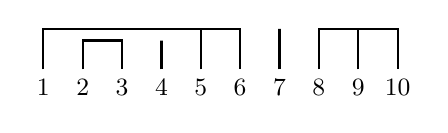
\begin{tikzpicture}[thick,font=\small]
 \path 	(0,0) 		node (a) {1}
 	(0.5,0) 	node (b) {2}
 	(1,0) 		node (c) {3}
 	(1.5,0) 	node (d) {4}
 	(2,0) 		node (e) {5}
 	(2.5,0) 	node (f) {6}
 	(3,0) 		node (g) {7}
 	(3.5,0) 	node (h) {8}
 	(4,0) 		node (i) {9}
 	(4.5,0) 	node (j) {10};
 \draw (a) -- +(0,0.75) -| (f);
 \draw (e) -- +(0,0.75) -| (e);
 \draw (b) -- +(0,0.60) -| (c);
 \draw (d) -- +(0,0.60) -| (d);
 \draw (g) -- +(0,0.75) -| (g);
 \draw (h) -- +(0,0.75) -| (j);
 \draw (i) -- +(0,0.75) -| (i);
 \end{tikzpicture}
\end{minipage}
\caption{Decorated Schr\"oder tree $t \otimes a_1\cdots a_{10}$ (left). The associated noncrossing partition of $t$ is $\pi(t) = \{\{ 1,5,6\},\{2,3\},\{4\}, \{7\}, \{8,9,10\}\}$ (right). }\label{fig:DecSchTree}
\end{figure}

Hence \eqref{eq:coproductH} also defines a coproduct $\delta_\A$ in $\cHS(\A)$ with the additional rule of carrying the decorations of the subtrees obtained in $R_c(t)$ and $P_c(t)$:
\[
	\delta_{\A} (t\otimes w)= \sum_{c\in \operatorname{Adm}(t)} R_c(t\otimes w)\otimes P_c(t\otimes w).
\]

\begin{Example}
Considering the decoration $a_1a_2a_3\in \A^{\otimes 3}$ of the Schr\"oder tree in Example \ref{ex:schrodertree}, we have the following computation of the coproduct in $H_{\mathcal{S}}(\mathcal{A})$:
\begin{align*}
\delta_\A \bigg( \begin{tikzpicture}[baseline={([yshift=-1.4ex]current bounding box.center)},scale=0.6,
level 1/.style={level distance=8mm,sibling distance=24mm},
level 2/.style={level distance=8mm,sibling distance=12mm},
]
\node(0)[solid node,label=above:{}]{}
child{node(1)[solid node]{}
	child{[black] node(112)[hollow node]{}}
		child{[black] node(1112)[hollow node]{}}
	}
child{node(2)[solid node]{}
	child{[black] node(11)[hollow node]{}
	}
	child{[black] node(111)[hollow node]{}
	}
};
\path (112) -- node {$a_1$} (1112);
\path (1112) -- node {$a_2$} (11);
\path (11) -- node {$a_3$} (111);
\end{tikzpicture}
\bigg)={} &\begin{tikzpicture}[scale=0.6,
level 1/.style={level distance=7mm,sibling distance=7mm}]
\node(0)[hollow node,label=above:{}]{};\end{tikzpicture} \otimes \begin{tikzpicture}[baseline={([yshift=-1ex]current bounding box.center)},scale=0.6,
level 1/.style={level distance=8mm,sibling distance=24mm},
level 2/.style={level distance=8mm,sibling distance=12mm},
]
\node(0)[solid node,label=above:{}]{}
child{node(1)[solid node]{}
	child{[black] node(112)[hollow node]{}}
		child{[black] node(1112)[hollow node]{}}
	}
child{node(2)[solid node]{}
	child{[black] node(11)[hollow node]{}
	}
	child{[black] node(111)[hollow node]{}
	}
};
\path (112) -- node {$a_1$} (1112);
\path (1112) -- node {$a_2$} (11);
\path (11) -- node {$a_3$} (111);
\end{tikzpicture} + \begin{tikzpicture}[baseline={([yshift=-1ex]current bounding box.center)},scale=0.6,
level 1/.style={level distance=8mm,sibling distance=24mm},
level 2/.style={level distance=8mm,sibling distance=12mm},
]
\node(0)[solid node,label=above:{}]{}
child{node(1)[solid node]{}
	child{[black] node(112)[hollow node]{}}
		child{[black] node(1112)[hollow node]{}}
	}
child{node(2)[solid node]{}
	child{[black] node(11)[hollow node]{}
	}
	child{[black] node(111)[hollow node]{}
	}
};
\path (112) -- node {$a_1$} (1112);
\path (1112) -- node {$a_2$} (11);
\path (11) -- node {$a_3$} (111);
\end{tikzpicture} \otimes \begin{tikzpicture}[scale=0.6,
level 1/.style={level distance=7mm,sibling distance=7mm}]
\node(0)[hollow node,label=above:{}]{};\end{tikzpicture} + \begin{tikzpicture}[baseline={([yshift=-1ex]current bounding box.center)},scale=0.6,
level 1/.style={level distance=8mm,sibling distance=14mm},
]
\node(0)[solid node,label=above:{}]{}
child{node(1)[hollow node]{}
	}
child{node(2)[solid node]{}
child{[black] node(11)[hollow node]{}
	}
	child{[black] node(111)[hollow node]{}
	}
};
\path (1) -- node {$a_2$} (11);
\path (11) -- node {$a_3$} (111);
%%as
\end{tikzpicture}\otimes \begin{tikzpicture}[baseline={([yshift=-1ex]current bounding box.center)},scale=0.6,
level 1/.style={level distance=8mm,sibling distance=12mm},
]
\node(0)[solid node,label=above:{}]{}
child{node(1)[hollow node]{}
	}
child{node(2)[hollow node]{}
};
\path (1) -- node {$a_1$} (2);
\end{tikzpicture} \\ &{} + \begin{tikzpicture}[baseline={([yshift=-1ex]current bounding box.center)},scale=0.6,
level 1/.style={level distance=8mm,sibling distance=14mm},
]
\node(0)[solid node,label=above:{}]{}
child{node(1)[solid node]{}
	child{[black] node(11)[hollow node]{}
	}
	child{[black] node(111)[hollow node]{}
	}
	}
child{node(2)[hollow node]{}
};
\path (11) -- node {$a_1$} (111);
\path (111) -- node {$a_2$} (2);
\end{tikzpicture}\otimes \begin{tikzpicture}[baseline={([yshift=-1ex]current bounding box.center)},scale=0.6,
level 1/.style={level distance=8mm,sibling distance=12mm},
]
\node(0)[solid node,label=above:{}]{}
child{node(1)[hollow node]{}
	}
child{node(2)[hollow node]{}
};
\path (1) -- node {$a_3$} (2);
\end{tikzpicture} + \begin{tikzpicture}[baseline={([yshift=-1ex]current bounding box.center)},scale=0.6,
level 1/.style={level distance=8mm,sibling distance=12mm},
]
\node(0)[solid node,label=above:{}]{}
child{node(1)[hollow node]{}
	}
child{node(2)[hollow node]{}
};
\path (1) -- node {$a_2$} (2);
\end{tikzpicture} \otimes \begin{tikzpicture}[baseline={([yshift=-1ex]current bounding box.center)},scale=0.6,
level 1/.style={level distance=8mm,sibling distance=12mm},
]
\node(0)[solid node,label=above:{}]{}
child{node(1)[hollow node]{}
	}
child{node(2)[hollow node]{}
};
\path (1) -- node {$a_1$} (2);
\end{tikzpicture} \;\begin{tikzpicture}[baseline={([yshift=-1ex]current bounding box.center)},scale=0.6,
level 1/.style={level distance=8mm,sibling distance=12mm},
]
\node(0)[solid node,label=above:{}]{}
child{node(1)[hollow node]{}
	}
child{node(2)[hollow node]{}
};
\path (1) -- node {$a_3$} (2);
\end{tikzpicture} .
\end{align*}
\end{Example}

We also have a grading inherited by $\cHS$ and the counit $\varepsilon_\A\colon \cHS(\A)\to\mathbb{C}$ is provided by the algebra morphism such that
\[
	\varepsilon_\A(t\otimes w) =
		\begin{cases} 1
		& \text{if $t=\circ$ and $w=\uno$,}\\ 0 &\text{otherwise.}
		\end{cases}
\]
Since $\operatorname{\deg}(t) = n$ if $t\in \ST(n)$, i.e., if $t$ has $n+1$ leaves, we obtain again that $t\otimes w$ has degree 0 if and only if $t$ has one leaf and $w$ has length~0, and this happens if only if $t$ is a single-vertex tree decorated with the empty word. Thus, $0$-th degree component of $H_\mathcal{S}(\A) \cong \mathbb{C}$ and hence, $H_\mathcal{S}(\A)$ is connected. Therefore we obtain:

\begin{Theorem}[\cite{JMNT}]
$(\cHS(\A),\delta_{\A},\varepsilon_\A)$ is a connected graded Hopf algebra.
\end{Theorem}

An important feature of the previous Hopf algebra is that its coproduct can be split into two half-coproducts in order to endow $\cHS(\A)$ with an unshuffle bialgebra structure. This splitting is described in the following way: Let $\cHS^+(\A)$ be the augmentation ideal of $\cHS(\A)$ and $t\otimes w \in \cHS^+$ a decorated Schr\"oder tree. We consider the subset of admissible cuts of a Schr\"oder tree given by
\[
	\operatorname{Adm}_\prec(t) := \{c\in \operatorname{Adm}(t)\colon \text{$R_c(t)$ contains the leftmost leaf of $t$}\}.
\]
We define the maps
\[
	\delta^+_{\prec,\A} (t\otimes w)= \sum_{c\in \operatorname{Adm}_\prec(t)} R_c(t\otimes w)\otimes P_c(t\otimes w),
\]
and
\[
	\delta_{\succ,\A}^+(t\otimes w) = \delta_\A(t\otimes w) - \delta_{\prec,\A}^+(t\otimes w).
 \]
These maps extend to $\delta_{\prec,\A},\delta_{\succ,\A} \colon \cHS^+(\A) \to \cHS(\A)\otimes \cHS(\A)$ by
\begin{align*}
	\delta_{\prec,\A}\big((t_1\otimes w_1)\cdots (t_m\otimes w_m)\big)
	&= \delta_{\prec,\A}(t_1\otimes w_1)\delta_\A\big((t_2\otimes w_2)\cdots (t_m\otimes w_m)\big),\\
	\delta_{\succ,\A}\big((t_1\otimes w_1)\cdots (t_m\otimes w_m)\big)
	&= \delta_{\succ,\A}(t_1\otimes w_1)\delta_\A\big((t_2\otimes w_2)\cdots (t_m\otimes w_m)\big).
\end{align*}
The precise statement of the new structure on $\cHS(\A)$ is as follows.

\begin{Theorem}[\cite{JMNT}]
$(\cHS(\A),\delta_{\prec,\A},\delta_{\succ,\A})$ is an unshuffle bialgebra.
\end{Theorem}

\begin{Remark}
In \cite{JMNT}, the authors give the definition of $\operatorname{Adm}_\prec(t)$ considering the rightmost leaf of $t$ instead of the leftmost one. Both structures are clearly isomorphic by considering the reversal of words $a_1\cdots a_n \in \A^{\otimes n}\mapsto a_n\cdots a_1 \in \A^{\otimes n}$.
\end{Remark}

Let $\A$ be an algebra. With the above theorem, we now have two unshuffle bialgebras $T(T_+(\A))$ and $\cHS(\A)$. The relation between both unshuffle bialgebras has been described in~\cite{JMNT} in terms of an algebra morphism which respects both coalgebra and unshuffle bialgebra structures. More precisely:

\begin{Theorem}[\cite{JMNT}]
Let $\iota\colon T(T_+(\A))\to \cHS(\A)$ be the algebra morphism defined by
\begin{equation}\label{eq:iota}
	\iota(w) = \sum_{t\in \ST(n)} t\otimes w,
\end{equation}
for any word $w= a_1\cdots a_n \in T_+(\A)$. Then $\iota$ is a coalgebra morphism and an unshuffle bialgebra morphism.
\end{Theorem}


\section{Monotone cumulants in terms of moments via Schr\"oder trees}\label{sec:monotone}

After having introduced the appropriate tools for our approach, we are prepared to attack the problem of finding a formula to express monotone cumulants in terms of moments.

 We begin with a noncommutative probability space $(\A,\varphi)$. By taking the algebra $\A$, we can consider both Hopf algebras $T(T_+(\A))$ and $\cHS(\A)$ described in Sections \ref{sec:shuffle} and \ref{sec:schroder}. We extend the linear functional $\varphi$ to a character $\Phi\colon T(T_+(\A))\to\mathbb{C}$ as it is done in Theorem \ref{thm:linkNCP}. Observe that we also have the notions of characters and infinitesimal characters on $\cHS(\A)$ defined in a~way analogous to the case of the Hopf algebra $T(T_+(\A))$. Hence we consider the following lifting of~$\varphi$ to a character $\tilde\Phi\colon \cHS(\A)\to\mathbb{C}$ by defining $\tilde\Phi(\circ) =1$ and
\begin{equation}
\label{eq:tildephi}
	\tilde\Phi(t \otimes a_1\cdots a_n)
	= \begin{cases} \varphi(a_1\cdots a_n) & \text{if $t$ is a corolla with $n+1$ leaves},\\ 0& \text{otherwise}. \end{cases}
\end{equation}
By using the coalgebra morphism $\iota$ defined in \eqref{eq:iota}, it is straightforward to see that $\Phi = \tilde\Phi \circ \iota.$ In addition, let $\tilde \rho\colon \cHS(\A)\to\mathbb{C}$ be the infinitesimal character such that $\tilde\Phi = \exp^*(\tilde\rho)$, where in this case $*$ stands for the convolution product defined in $\operatorname{Lin}(\cHS(\A),\mathbb{C})$. As stated in the following result, we can relate $\tilde\rho$ with the monotone cumulants on $\A$.

\begin{Proposition}\label{prop:easy}
Let $\rho\colon T(T_+(\A))\to\mathbb{C}$ be defined by $\rho = \tilde\rho\circ\iota$. Then $\rho$ is a infinitesimal character such that $\Phi = \exp^*(\rho).$
\end{Proposition}

\begin{proof}Since $\iota$ is an algebra morphism and $\tilde\rho$ is an infinitesimal character over $\cHS(\A)$, for any words $w_1,w_2\in T(T_+(\A))$ we have
\[
	\rho(w_1|w_2) = \tilde\rho(\iota(w_1|w_2)) = \tilde\rho(\iota(w_1)\iota(w_2)) = 0.
\]
Furthermore, since $\iota$ is also a coalgebra morphism, we obtain that for any $w\in T_+(\A)$
\[
	\Phi(w) = \big(\tilde\Phi \circ\iota\big)(w)
	= \tilde\Phi(\iota(w))
	= \exp^*(\tilde \rho)(\iota(w)) = \exp^*(\tilde\rho\circ\iota)(w)
	= \exp^*(\rho)(w).
\]
Note that we used that $\iota$ is a coalgebra morphism in the fourth equality.
\end{proof}

By the above proposition and Theorem \ref{thm:linkNCP}, we conclude that if $w=a_1\cdots a_n$, then
\begin{equation}
\label{eq:rhoiota}
\rho(w) = \sum_{t\in \ST(n)} \tilde{\rho}(t\otimes w)
\end{equation}
is the infinitesimal character associated to the monotone cumulants of $a_1,\dots,a_n\in \A$. On the other hand, note that
\[
	\tilde\Phi
	= \exp^*(\tilde\rho) \ \Leftrightarrow \ \tilde\rho
	= \log^*\big(\tilde\Phi\big)
	= \log^*\big(\varepsilon + \big(\tilde\Phi - \varepsilon\big)\big)
	= \sum_{k=1}^\infty \frac{(-1)^{k+1}}{k} \hat\Phi^{* k},
\]
where $\hat\Phi = \tilde\Phi - \varepsilon$. In order to find an expression for the $k$-fold convolution product $\hat\Phi^{*k}$, we will need to describe the so-called Murua coefficients.


\subsection{Murua coefficients}
\label{ssec:Murua}

Recall that given a forest of planar rooted trees, we have a poset structure canonically associated to it. The following coefficients associated to rooted trees have appeared in the analysis of the continuous Baker--Campbell--Hausdorff problem in a Hall basis (see Murua's article~\cite{Murua}).

\begin{Definition}
Let $t$ be a planar rooted tree seen as a poset with $n = |t|$ vertices. For any integer $0 < k< n+1$, we denote by $\omega_k(t)$ to the number of surjective functions $f\colon t\to \{1,\dots,k\}$ such that for any two vertices $v$, $w$ in $t$ with $v<w$, we have that $f(v)<f(w)$. We then define the quantity $\omega(t)$ by
\begin{equation}\label{eq:muruacoeff}
\omega(t) = \sum_{k=1}^n \frac{(-1)^{k+1}}{k} \omega_k(t).
\end{equation}
If $f$ is a forest with trees $t_1,\dots, t_m$, we define $\omega(f) = \omega(t_1)\cdots \omega(t_m).$
\end{Definition}
